%% abtex2-modelo-relatorio-tecnico.tex, v-1.9.7 laurocesar
%% Copyright 2012-2018 by abnTeX2 group at http://www.abntex.net.br/ 
%% 
%% This work may be distributed and/or modified under the
%% conditions of the LaTeX Project Public License, either version 1.3
%% of this license or (at your option) any later version.
%% The latest version of this license is in
%% http://www.latex-project.org/lppl.txt
%% and version 1.3 or later is part of all distributions of LaTeX
%% version 2005/12/01 or later.
%% 
%% This work has the LPPL maintenance status `maintained'.
%% 
%% The Current Maintainer of this work is the abnTeX2 team, led
%% by Lauro César Araujo. Further information are available on 
%% http://www.abntex.net.br/
%% 
%% This work consists of the files abntex2-modelo-relatorio-tecnico.tex,
%% abntex2-modelo-include-comandos and abntex2-modelo-references.bib
%% 

% ------------------------------------------------------------------------
% ------------------------------------------------------------------------
% abnTeX2: Modelo de Relatório Técnico/Acadêmico em conformidade com 
% ABNT NBR 10719:2015 Informação e documentação - Relatório técnico e/ou
% científico - Apresentação
% ------------------------------------------------------------------------ 
% ------------------------------------------------------------------------

\documentclass[
% -- opções da classe memoir --
12pt,				% tamanho da fonte
openright,			% capítulos começam em pág ímpar (insere página vazia caso preciso)
oneside,			% para impressão em recto e verso. Oposto a oneside
a4paper,			% tamanho do papel. 
% -- opções da classe abntex2 --
% chapter=TITLE,		% títulos de capítulos convertidos em letras maiúsculas
% section=TITLE,		% títulos de seções convertidos em letras maiúsculas
% subsection=TITLE,	% títulos de subseções convertidos em letras maiúsculas
% subsubsection=TITLE,% títulos de subsubseções convertidos em letras maiúsculas
% -- opções do pacote babel --
english,			% idioma adicional para hifenização
french,				% idioma adicional para hifenização
spanish,			% idioma adicional para hifenização
brazil,				% o último idioma é o principal do documento
]{abntex2}


% ---
% PACOTES
% ---

% ---
% Pacotes fundamentais 
% ---
\usepackage{lmodern}			% Usa a fonte Latin Modern
\usepackage[T1]{fontenc}		% Selecao de codigos de fonte.
\usepackage[utf8]{inputenc}		% Codificacao do documento (conversão automática dos acentos)
\usepackage{indentfirst}		% Indenta o primeiro parágrafo de cada seção.
\usepackage{color}				% Controle das cores
\usepackage{graphicx}			% Inclusão de gráficos
\usepackage{microtype} 			% para melhorias de justificação
\usepackage{gensymb}
% ---

% ---
% Pacotes adicionais, usados no anexo do modelo de folha de identificação
% ---
\usepackage{multicol}
\usepackage{multirow}
% ---

% ---
% Pacotes adicionais, usados apenas no âmbito do Modelo Canônico do abnteX2
% ---
\usepackage{lipsum}				% para geração de dummy text
% ---

% ---
% Pacotes de citações
% ---
\usepackage[brazilian,hyperpageref]{backref}	 % Paginas com as citações na bibl
\usepackage[alf]{abntex2cite}	% Citações padrão ABNT

% --- 
% CONFIGURAÇÕES DE PACOTES
% --- 

% ---
% Configurações do pacote backref
% Usado sem a opção hyperpageref de backref
\renewcommand{\backrefpagesname}{Citado na(s) página(s):~}
% Texto padrão antes do número das páginas
\renewcommand{\backref}{}
% Define os textos da citação
\renewcommand*{\backrefalt}[4]{
	\ifcase #1 %
  Nenhuma citação no texto.%
	\or
  Citado na página #2.%
	\else
  Citado #1 vezes nas páginas #2.%
	\fi}%
% ---

% ---
% Informações de dados para CAPA e FOLHA DE ROSTO
% ---
\titulo{Interferência Ótica}
\autor{Amanda Cabral, Camila Oliveira, Pedro Branquinho}
\local{Lorena, São Paulo}
\data{2019}
\instituicao{%
  Universidade de São Paulo -- USP
  \par
  Escola de Engenharia de Lorena
  \par
  Ciências Básicas e Ambiental}
\tipotrabalho{Relatório técnico de Física Experimental}
% O preambulo deve conter o tipo do trabalho, o objetivo, 
% o nome da instituição e a área de concentração 
\preambulo{Experimentos número 6}
% ---

% ---
% Configurações de aparência do PDF final

% alterando o aspecto da cor azul
\definecolor{blue}{RGB}{41,5,195}

% informações do PDF
\makeatletter
\hypersetup{
  % pagebackref=true,
  pdftitle={\@title}, 
  pdfauthor={\@author},
  pdfsubject={\imprimirpreambulo},
  pdfcreator={LaTeX with abnTeX2},
  pdfkeywords={abnt}{latex}{abntex}{abntex2}{relatório técnico}, 
  colorlinks=true,       		% false: boxed links; true: colored links
  linkcolor=blue,          	% color of internal links
  citecolor=blue,        		% color of links to bibliography
  filecolor=magenta,      		% color of file links
  urlcolor=blue,
  bookmarksdepth=4
}
\makeatother
% --- 

% --- 
% Espaçamentos entre linhas e parágrafos 
% --- 

% O tamanho do parágrafo é dado por:
\setlength{\parindent}{1.3cm}

% Controle do espaçamento entre um parágrafo e outro:
\setlength{\parskip}{0.2cm}  % tente também \onelineskip

% ---
% compila o indice
% ---
\makeindex
% ---

% ----
% Início do documento
% ----
\begin{document}

% Seleciona o idioma do documento (conforme pacotes do babel)
% \selectlanguage{english}
\selectlanguage{brazil}

% Retira espaço extra obsoleto entre as frases.
\frenchspacing 

% ----------------------------------------------------------
% ELEMENTOS PRÉ-TEXTUAIS
% ----------------------------------------------------------
% \pretextual

% ---
% Capa
% ---
\imprimircapa
% ---

% ---
% Folha de rosto
% (o * indica que haverá a ficha bibliográfica)
% ---
\imprimirfolhaderosto*
% ---


% ---
% RESUMO
% ---

% resumo na língua vernácula (obrigatório)
\setlength{\absparsep}{18pt} % ajusta o espaçamento dos parágrafos do resumo
\begin{resumo}
Por meio de um elaborado aparato experimental, utilizando-se diversas lentes,
conseguimos com que a luz vermelha ficasse em condições nítidas de
interferência. Por conseguinte, demonstramos o caracter de onda das ondas
eletromagnéticas.
  
  \noindent
  \textbf{Palavras-chaves}: Interferência; Onda eletromagnética.
\end{resumo}
% ---

% ---
% inserir lista de ilustrações
% ---
\pdfbookmark[0]{\listfigurename}{lof}
\listoffigures*
\cleardoublepage
% ---

% ---
% inserir lista de tabelas
% ---
\pdfbookmark[0]{\listtablename}{lot}
\listoftables*
\cleardoublepage
% ---


% ---
\pdfbookmark[0]{\contentsname}{toc}
\tableofcontents*
\cleardoublepage
% ---


% ----------------------------------------------------------
% ELEMENTOS TEXTUAIS
% ----------------------------------------------------------
\textual

% ----------------------------------------------------------
% Introdução (exemplo de capítulo sem numeração, mas presente no Sumário)
% ----------------------------------------------------------
\chapter[Objetivo]{Objetivo}

O aparato experimental foi feito especialmente para que um feixe de luz se
comportasse como duas fontes. E, à partir disso, impomos a condição, por meio do
aparato experimental, de que esses dois feixes de luz se encontrassem. E, então
magnificamos o que acontece em escalas microscópicas, exatamente no ponto de
encontro dos feixes. Por fim, objetivamos mostrar que há interferência, e que a
superposição é válida, assim, mostrando-se que
essa luz possui comportamento ondular, como previsto na literatura \cite{rubinowicz1957}.

\chapter[Introdução]{Introdução Teórica}

O estudo da luz originou-se em uma série de experimentos no séculos XVII, XVIII
e XIX, com Francesco Grimaldi, Isaac Newton, Thomas Young e Augustin-Jean Fresnel.
Isaac Newton acreditava, pelo resultado dos seus experimentos, que a luz branca
deveria ser composta por corpúsculos, pois viajam em linha reta, e podem ser
refratados. Vemos alguns de seus experimentos, esquematicamente, na \autoref{img:n1} e \autoref{img:n2}.

\begin{figure}[!htb]
	\caption{\label{img:n1} Experimento, com prismas, de Newton}
	\begin{center}
	  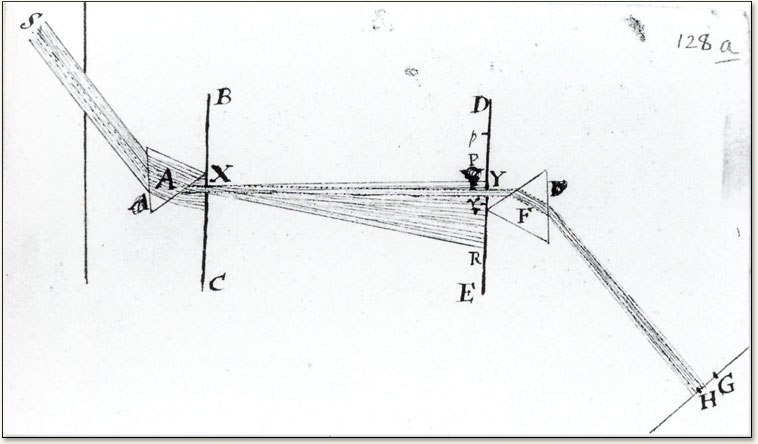
\includegraphics[scale=0.3]{./imagens/n1.jpg}
	\end{center}
	\legend{Fonte: http://www.webexhibits.org/colorart/bh.html}
\end{figure}

\begin{figure}[!htb]
	\caption{\label{img:n2} Representação moderna do experimental de Newton}
	\begin{center}
	  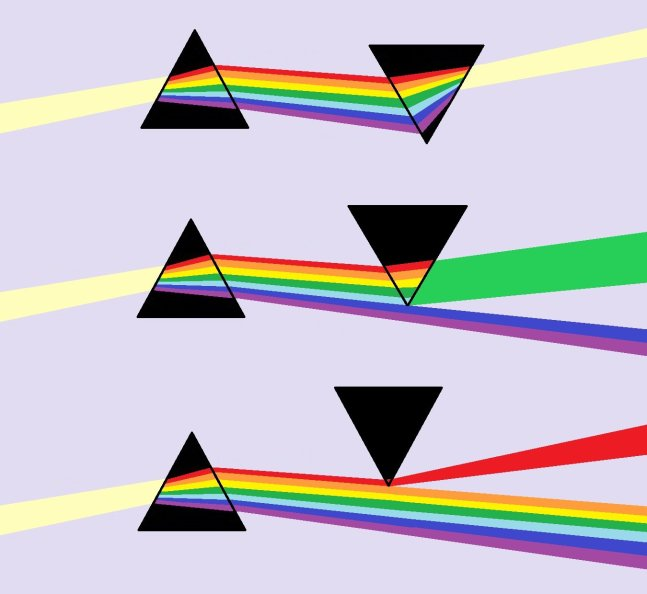
\includegraphics[scale=0.3]{./imagens/n2.jpg}
	\end{center}
	\legend{Fonte: Helen Klus, http://www.thestargarden.co.uk/Newtons-theory-of-light.html}
\end{figure}

\clearpage


Porém, T. Young especulava, à partir de conhecimentos físicos, e situações
hipotéticas de que a luz deveria se comportar como onda, sob certas condições.
Em seu livro, \textit{A course of lectures on natural philosophy and the mechanical
  arts: in two volumes}, Young descreve experimentos para que seja observada a
natureza ondular da luz \cite{young1807}. Podemos ver uma das imagens em seu
livro, descrevendo um experimento de interferência na \autoref{img:y1}.

\begin{figure}[!htb]
	\caption{\label{img:y1} Experimento sobre interferência ondular de Young}
	\begin{center}
	  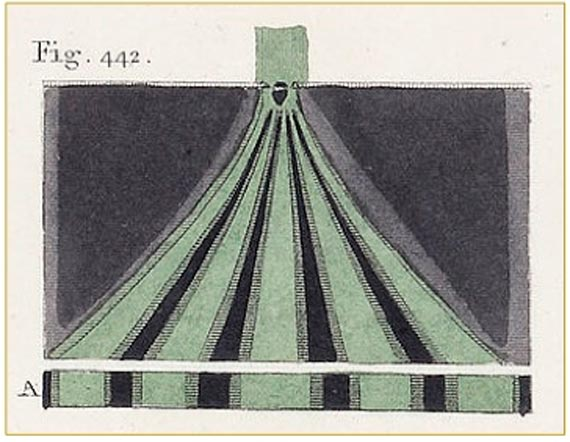
\includegraphics[scale=0.3]{./imagens/y1.jpg}
	\end{center}
	\legend{Fonte: \textit{A course of lectures on natural philosophy and the mechanical
  arts: in two volumes}}
\end{figure}

Iremos utilizar, para a medida da distância entre duas interferências
contrutivas, consecutivas, a fórmula,

$$ \Lambda = \frac{\lambda}{2 \sin{(\frac{\theta}{2})}}
\label{eqn:Lambda}$$

\cite{ifsc2013}.

\chapter{Procedimento Experimental}

\begin{enumerate}
  
\item Utilizou-se um laser e um divisor de feixe e ajustou-o de tal forma que os dois feixes
  emergentes estivessem aproximadamente paralelos entre si, horizontais, e
  separados por $\approx$2 cm. Com isso, produziu-se uma diferença de caminho óptico entre
  dois feixes provenientes de uma mesma fonte corrente (laser de He/Ne)
\item Posicionou-se quatro espelhos (planos) sobre a bancada para que o feixe principal
  percorra $\approx$5 metros antes de iluminar o centro de uma escala micrométrica,
  posicionada no centro da bancada. Ajustou-se os espelhos (altura e inclinação) para
  que o feixe incidisse próximo ao centro dos espelhos e estivesse sempre horizontal,
  mantendo a mesma altura em relação à bancada. Bloqueou-se o feixe secundário do
  divisor para não se confundir durante esse alinhamento.
\item Posicionou-se um espelho plano para que o feixe transmitido através da escala
  micrométrica percorresse $\approx$2m até o centro de um anteparo, mantendo-se sempre
  no plano horizontal
\item Posicionou-se uma lente de distância focal 5 ou 6 cm após a escala micrométrica de
  tal forma que esta esteja próxima ao foco da lente. Ajustou-se lateralmente a lente,
  de modo que o feixe do laser passasse pelo seu centro. Nessa condição, a parte
  mais brilhante do feixe ampliado deve estar centralizado no anteparo. Observou-se a
  imagem da escala micrométrica projetada no anteparo.
\item Desbloqueou-se o feixe secundário do divisor de feixes e ajustou-se a orientação do
  espelho 100\% refletor do divisor de modo que os dois feixes pudessem se superpor
  na escala micrométrica. Fez-se o ajuste fino observando o aparecimento de um
  padrão de interferência nítido no anteparo.
\item Mediu-se a distância percorrida pela feixe entre o divisor de feixes e a escala
  micrométrica e a separação de feixes no divisor. Com isso determinou o ângulo
  entre os feixes.
\item Realizou-se a medida da separação entre máximos consecutivos e calculou-se o
  comprimento de onda do laser. Repetiu-se para mais duas separações entre os
  feixes após o divisor, preenchendo a tabela dada.
\item Focalizou-se nitidamente o retículo, medindo a distância lente-retículo (S) e
  lente-anteparo (S’), e a distância entre máximos no anteparo. Com isso, calculou-se
  a separação entre máximos no retículo e determinou-se o comprimento de onda do
  laser. Repetiu-se para mais duas separações entre os espelhos.

\end{enumerate}

\clearpage

\chapter{Resultados}

Primeiramente definimos o valor de $\theta$, que é dado pelo $\arctan{(\frac{D}{5m})}$, pela relação trigonométrica de triângulos retângulos. Na
\autoref{img:fig1} é possível ver que a distância do semiespelho até a escala
micrométrica é um dos catetos do triângulo, e a distância entre os dois espelhos
é o outro cateto.

\begin{figure}[!htb]
	\caption{\label{img:fig1} Representação do aparato experimental}
	\begin{center}
	  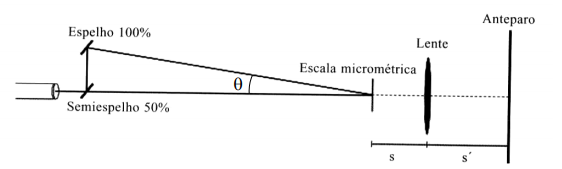
\includegraphics[scale=1]{./imagens/fig1.png}
	\end{center}
	\legend{Fonte: Os autores}
\end{figure}

As tabelas dos dados referentes à esse aparato experimental,
\begin{table}[htb]
  \IBGEtab{%
    \caption{Memória de cálculo}
    \label{tab:Mem}
  }
  {%
    \begin{tabular}{cccc}
      \toprule
      D(m) & $\tan{O} = \frac{D}{5}$ & O & $2 \sin{(2 O)}$ \\
      \midrule \midrule
      0.0136 & 0.00272 & 0.155844 & 0.01879 \\
      \hline
      0.0103 & 0.00206 & 0.118029 & 0.008239 \\
      \hline
      0.012 & 0.00240 & 0.137509 & 0.009599 \\
      \bottomrule
    \end{tabular}%
  }
  {%
    \fonte{Produzido pelos autores}%
  }
\end{table}


\begin{table}[htb]
  \IBGEtab{%
    \caption{\label{tab:Sep}Tabela com os valores de separação lateral medidos por uma escala milimétrica}%
  }
  {%
    \begin{tabular}{cccccc}
      \toprule
      \multicolumn{4}{c}{Separação lateral entre os feixes (cm)} & Distância entre os máximos (mm) & Comprimento de ondas (nm) \\
      \midrule \midrule
      $d_{1}$ & $d_{2}$ & $d_{3}$& $d_{4}$& ~ &  ~ \\
      \hline
      1.4 & 1.4 & 1.3 & 1.360 & 0.3 & 3263.48 \\
      \hline
      1 & 0.9 & 1.2 & 1.103 & 0.2& 1647.99 \\
      \hline
      1.200& 1.200& 1.200 & 1.200 & 0.25&  2399.98 \\
      \hline
      \multicolumn{6}{c}{$\lambda = 2437.15 \pm 660.4 nm$}\\
      \bottomrule
    \end{tabular}%
  }
  {%
    \fonte{Produzido pelos autores}%
  }
\end{table}



Para calcular a distância entre o comprimento de onda utilizamos a \autoref{eqn:Lambda}, onde pegamos o valor do $\theta$ calculado anteriormente e utilizamos o valor da
separação lateral entre os pontos de máximo $\Lambda$, \autoref{eqn:Lambda}.
 

Para medir a distância lateral entre os máximos nessa parte do experimento
utilizamos a escala micrométrica, e os valores obtidos são apresentados na \autoref{tab:Sep}.


O primeiro método para se obter o valor de $\lambda$ foi o menos preciso pois o seu desvio padrão foi bem grande e o menos exato considerando a que o valor médio experimental está muito distante do valor real conhecido. O segundo método foi mais preciso com o valor do desvio padrão menor, mas ainda assim não é exato pois o valor médio experimental ser muito superior ao valor real. 


Na segunda parte do experimento, utilizamos o artifício da ampliação lateral
feita com uma lente, calculamos o valor da ampliação M, que é dado pela
razão entre a distância da lente até o objeto e a distância da imagem até a
lente, e depois com o valor da ampliação e o valor do tamanho lateral da
imagem, calculamos o valor do tamanho lateral do objeto, que é equivalente a
distância entre dois máximos, que são aprensetados na \autoref{tab:Sep}.

\begin{table}[!htb]
  \IBGEtab{%
    \caption{\label{tab:Sep}Tabela com os valores de separação lateral medidos por uma escala micrométrica}%
 
  }
  {%
    \begin{tabular}{ccccccc}
      \toprule
      \multicolumn{4}{c}{Separação lateral entre feixes (cm)} & Distância entre máximos (mm) & $\frac{S}{S'}$ & Comprimento de ondas (nm) \\
      \midrule \midrule
      $d_{1}$ & $d_{2}$ & $d_{3}$& $ d_{4} $ & ~ & ~ &  ~\\
      \hline
      1.4 & 1.4 & 1.3 & 1.36 & 1.0 & 30.73 & 3263.49 \\
      \hline
      1 & 0.9 & 1.2 & 1.103 & 0.2& 30.73 & 536.28 \\
      \hline
      1.2& 1.2& 1.2  & 1.2 & 0.25& 30.73 & 780.99 \\
      \hline
      \multicolumn{6}{c}{$ \lambda = 2437.15$ $\pm$ $660.4 nm $}\\
      
      \bottomrule
    \end{tabular}%
  }
  {%
    \fonte{Produzido pelos autores}%
  }
\end{table}


\clearpage

\chapter{Conclusão}

No experimento esperávamos poder definir o comprimento de onda de uma luz polarizada. Contudo, devido a escala do resultado que esperávamos, que é muito pequena, e os diversos erros a serem considerados nas medidas de comprimento durante a atividade experimental, não conseguimos chegar a um resultado satisfatório próximo ao real.

\clearpage
% ---

\bibliography{ref-bib}

\end{document}
